%---------------------------------------------------------------------
\begin{frame}{A quick announcement: final exam date \& time}

    The \newbold{final exam} will take place on \newbold{Thursday May 7th from 9-11am}\\
    \vspace{10mm}

    $\implies$ Make \textbf{absolutely sure} to be available at that time!
\end{frame}
%---------------------------------------------------------------------
\begin{frame}{Previous classes on adverse selection}

    Einav and Finkelstein (2011) graphical framework
    \begin{itemize}
        \item Only premium varies across contracts:
        we held \textbf{other contract features fixed} (e.g., deductible, co-insurance rate, etc.)
    \end{itemize}
    \vspace{3mm}
    \pause

    In reality, insurance contracts differ along these other dimensions
    \begin{itemize}
        \item Different financial dimensions: deductible, coinsurance rate, etc.
        \item Narrow networks
        \item Different drug formularies: some plans cover some drugs while others do not
    \end{itemize}
    $\rightarrow$ Why do they differ?\\
    \vspace{3mm}
    \pause
     
    Today: can \newbold{adverse selection} impact \newbold{contract features}? \\
    \pause 
    $\rightarrow$A way to think about it: the \newbold{Rothschild-Stiglitz (1976)} model
    
\end{frame}
%---------------------------------------------------------------------
\begin{frame}{}
    \begin{center}
    \Large \textcolor{maroon}{The Rothschild-Stiglitz (1976) model}
    \end{center}
\end{frame}
%---------------------------------------------------------------------
\begin{frame}{Change the space: now we are in $(I_H, I_S)$ space}

    \begin{columns}[T]
        \begin{column}{0.56\textwidth}
            Denote $I$ the total income.\\
            The consumer can be:
            \begin{itemize}
                \item Healthy ($H$) $\rightarrow$ income $H_E$
                \item Sick ($S$) $\rightarrow$ income $S_E$
            \end{itemize}
            $\implies$ $(H_E, S_E)$ is the initial endowment point $E$.\\
            \vspace{2mm}     
            \only<2>{How to represent this into the $(I_H, I_S)$ space?}
        \end{column}
        \begin{column}{0.44\textwidth}
            \centering
            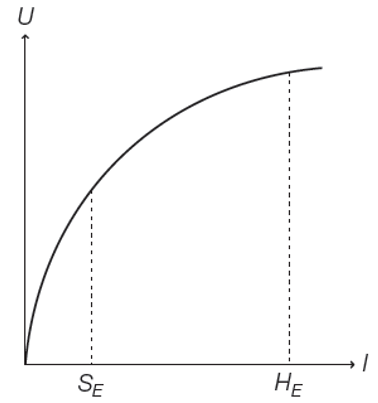
\includegraphics[width=\textwidth]{./input/BHT_fig91a.png}
        \end{column}
    \end{columns}

    
\end{frame}
%---------------------------------------------------------------------
\begin{frame}{Change the space: now we are in $(I_H, I_S)$ space}

    \centering
    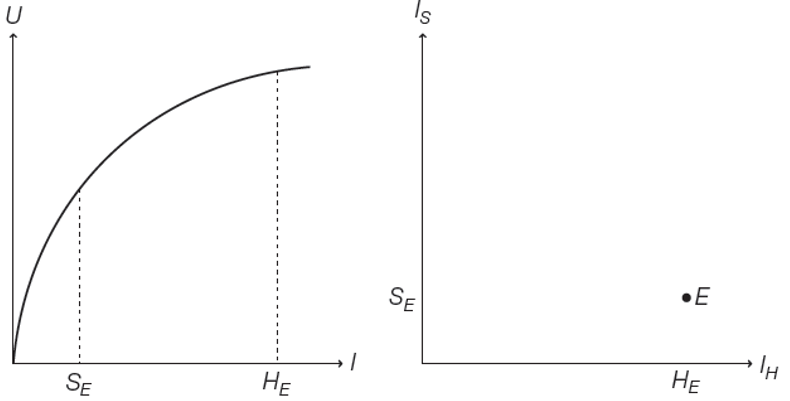
\includegraphics[width=\textwidth]{./input/BHT_fig91b.png}
    
\end{frame}
%---------------------------------------------------------------------
\begin{frame}{Moving across contracts in the $(I_H, I_S)$ space}

        A contract is offered at premium $r$: it gives an extra income $q$ when sick.\\
        \only<1>{\vspace{55mm}}
        \only<2>{$\rightarrow$ How to represent this contract in the $(I_H, I_S)$ space?\\
        \vspace{48mm}}
        \only<3>{
        $\rightarrow$ How to represent this contract in the $(I_H, I_S)$ space?\\
        \begin{center}
        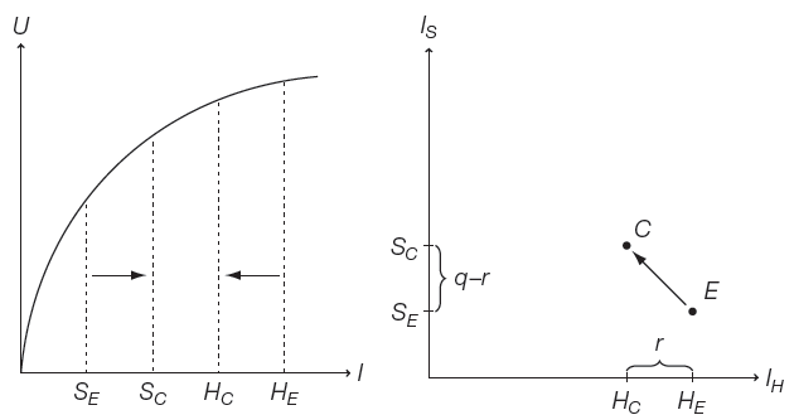
\includegraphics[width=0.85\textwidth]{./input/BHT_fig92.png}
        \end{center}
        }

\end{frame}
%---------------------------------------------------------------------
\begin{frame}{How to draw indifference curves in the $(I_H, I_S)$ space?}

    \begin{columns}[T]
        \begin{column}{0.56\textwidth}
            Indifference curves in the $(I_H, I_S)$ space:
            \begin{itemize}
                \item Downward sloping. \textit{Can you see why?}
                % Intuition: a contract that gives more income in both states has to be on a different indifference curve
                % Can verify mathematically with differential equations
                \item Risk-averse $\implies$ convex indifference curves. \textit{Can you see why?}
                % Intuition: as in general consumer theory where concave utility gives convex indifference curves,
                % here the consumer is risk-averse and thus prefers a more balanced contract (i.e., one that gives more similar income in both states) to a more unbalanced contract (i.e., one that gives much higher income in one state than in the other state)
                % mathematical proof dIs/dIH depends on curvature of U.
            \end{itemize}
            \only<1>{\vspace{48mm}}
        \end{column}
        \begin{column}{0.44\textwidth}
            \centering
            \only<2>{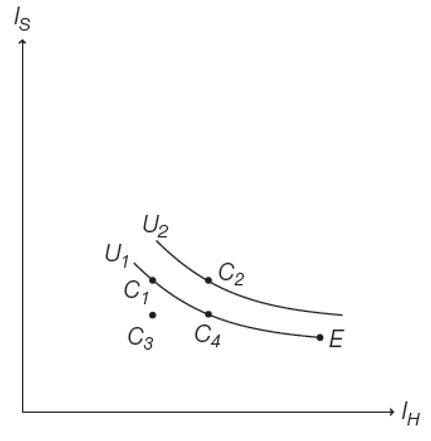
\includegraphics[width=\textwidth]{./input/BHT_fig94.png}}
        \end{column}
    \end{columns}
    
\end{frame}
%---------------------------------------------------------------------
\begin{frame}{The full insurance line}

    \begin{columns}[T]
        \begin{column}{0.56\textwidth}
            What does full insurance look like in the $(I_H, I_S)$ space?\\
            \only<2>{$\rightarrow$ The \newbold{full insurance line} is the 45 degree line, where $I_H = I_S$.}
            \only<1>{\vspace{48mm}}
        \end{column}
        \begin{column}{0.44\textwidth}
            \centering
            \only<2>{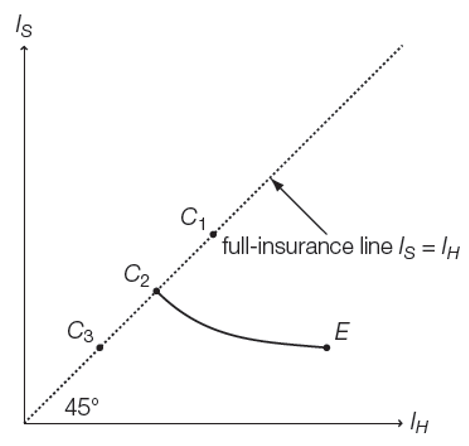
\includegraphics[width=\textwidth]{./input/BHT_fig95.png}}
        \end{column}
    \end{columns}
    %above 45degree line: more income when sick than when healthy
    %below 45degree line: more income when healthy than when sick
    
\end{frame}
%---------------------------------------------------------------------
\begin{frame}{The zero-profit line}

    Reminder: \newbold{actuarially fair contract} $\implies$ the contract such that the expected profit of the insurer is zero.\\
    \vspace{2mm}
    \pause

    Assume the probablity of being sick is $p$.\\
    Remember the consumer's endowment point $E = (H_E, S_E)$.\\
    % $H_E$ is income when healthy, $S_E$ is income when sick.\\
    \vspace{2mm}
    \pause

    Denote the contracts offered by the insurer $(I_H, I_S)$.\\
    %\textit{Note: this is expressed in income space, not in premium space.}\\
    \vspace{2mm}
    \pause

    What is the \newbold{expected profit of the insurer} from offering such contracts to consumer with endowment $E$?
    \begin{align*}
        \pi = p \underbrace{( S_E - I_S )}_{\text{payout net of premium } (-(q-r))} + (1-p) \underbrace{( H_E - I_H )}_{\text{premium: r}} 
    \end{align*}
\end{frame}
%---------------------------------------------------------------------
\begin{frame}{The zero-profit line}
    What is the \newbold{expected profit of the insurer} from offering such contracts to consumer with endowment $E$?
    \begin{align*}
        \pi = p \underbrace{( S_E - I_S )}_{\text{payout net of premium } (-(q-r))} + (1-p) \underbrace{( H_E - I_H )}_{\text{premium: r}} 
    \end{align*}
    \textit{Note: you can write it as $\pi = p (-(q-r))  + (1-p) r = r - pq $ (link to previous classes).}
    \vspace{2mm}
    \pause

    Actuarially fair premium: $\pi = 0$. We want to find an equation of $I_S$ as a function of $I_H$ such that $\pi = 0$.
    \begin{align*}
        0 &= p ( S_E - I_S ) + (1-p) ( H_E - I_H ) \\
        \implies I_S &= \frac{1-p}{p} ( H_E - I_H ) + S_E
    \end{align*}

\end{frame}
%---------------------------------------------------------------------
\begin{frame}{The zero-profit line}

    \begin{columns}[T]
        \begin{column}{0.56\textwidth}
            The \newbold{zero-profit line} is the set of contracts that give zero expected profit to the insurer:
            \begin{align*}
                I_S &= \frac{1-p}{p} ( H_E - I_H ) + S_E
            \end{align*}
            \only<1>{\vspace{43mm}}
        \end{column}
        \begin{column}{0.44\textwidth}
            \centering
            \only<2>{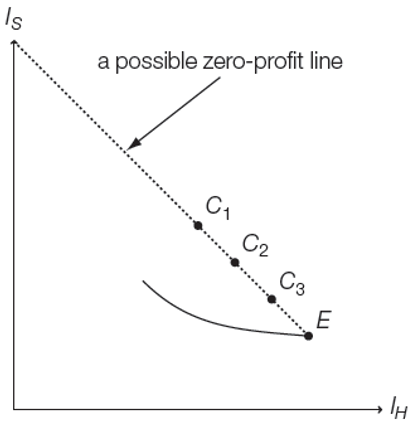
\includegraphics[width=\textwidth]{./input/BHT_fig96.png}}
        \end{column}
    \end{columns}

\end{frame}
%---------------------------------------------------------------------
\begin{frame}{The zero-profit line: profitable and unprofitable contracts}

    \centering
    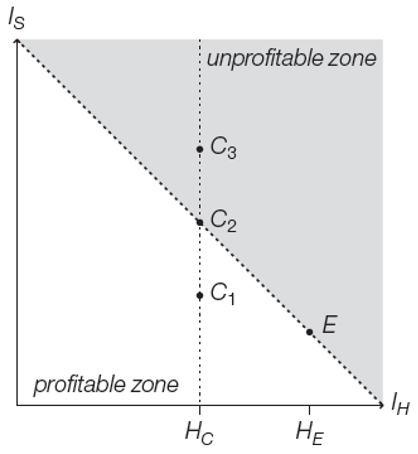
\includegraphics[width=0.5\textwidth]{./input/BHT_fig97.png}

\end{frame}
%---------------------------------------------------------------------
\begin{frame}{What are the feasible contracts?}

    \only<1>{}
    \only<2>{
    \begin{columns}[T]
        \begin{column}{0.56\textwidth}
        \begin{enumerate}
            \item Zone $R_1$: over full insurance. Implausible for risk-averse consumers.
            \item Zone $R_2$: below endowment point utility $\rightarrow$ consumers prefer endowment point
            \item Zone $R_3$: above zero-profit line $\rightarrow$ unprofitable for insurer
            \item Zone $F$: \newbold{feasible contracts}
        \end{enumerate}
        \end{column}
        \begin{column}{0.44\textwidth}
            \centering
            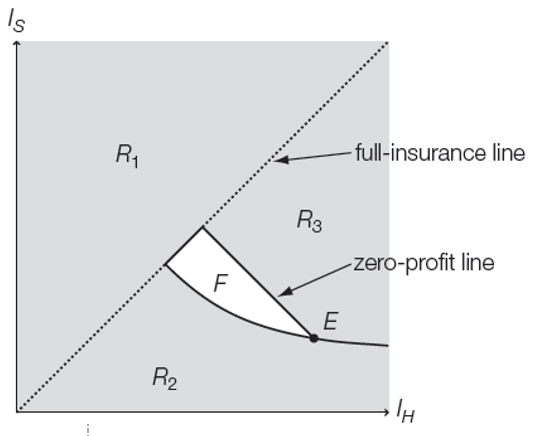
\includegraphics[width=1.1\textwidth]{./input/BHT_fig98.png}
        \end{column}
    \end{columns}
    }

\end{frame}
%---------------------------------------------------------------------
\begin{frame}{Equilibrium contracts}

    A \textbf{contract} is an \newbold{equilibrium} if
    \begin{enumerate}
        \item This contract offers the most utility to the consumer (compared to other existing contracts)
        \item The contract does not imply negative profits for the insurer
        \item No other contract can be offered that would give more utility to the consumer \textbf{and} give insurers at least zero profit
    \end{enumerate}

\end{frame}
%---------------------------------------------------------------------
\begin{frame}{$\alpha$ is \newbold{NOT} an equilibrium}

    \centering
    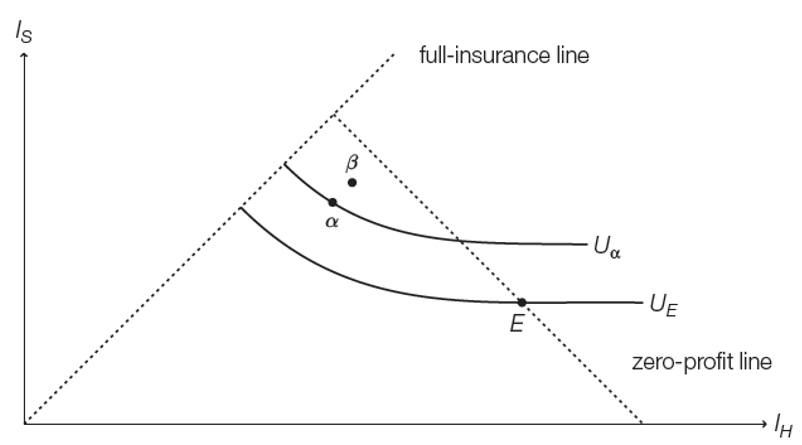
\includegraphics[width=0.7\textwidth]{./input/BHT_fig99.png}

    % beta gives positive profits to the insurer and all consumers woudl switch to it

\end{frame}
%---------------------------------------------------------------------
\begin{frame}{$\Omega$ is an equilibrium}

    \centering
    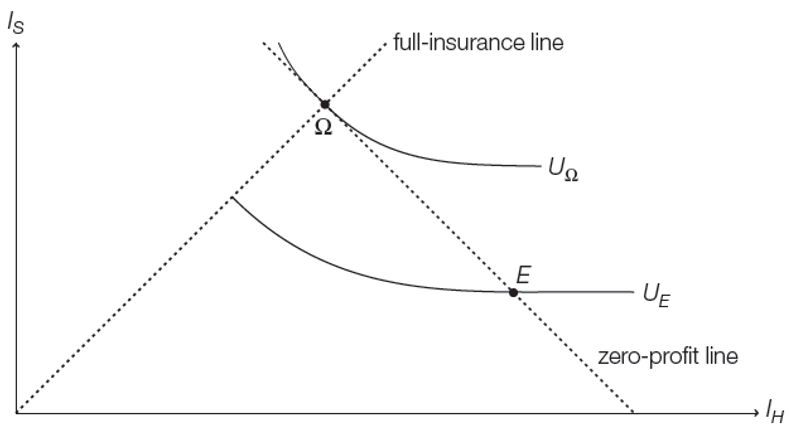
\includegraphics[width=0.7\textwidth]{./input/BHT_fig910.png}
    % Equilibrium here: full insurance contract with zero profits

\end{frame}
%---------------------------------------------------------------------
\begin{frame}{Introducing heterogeneity in consumers}

    We want to study \newbold{adverse selection} in the health insurance market\\
    $\rightarrow$ some consumers are more likely to be sick than others\\
    $\rightarrow$ consumers are \newbold{heterogeneous} in their probability of being sick\\
    \vspace{5mm}

    Introducing two types of consumers: \textbf{high risk} (frail) and \textbf{low risk} (robust)\\
    $\implies$ $p_F > p_R$\\
    \vspace{5mm}
    \textit{Note: we assume their utility functions are identical.\\
    They only differ in their risk profile through the probability to get sick.}

\end{frame}
%---------------------------------------------------------------------
\begin{frame}{Health insurers face different zero-profit lines}

    \centering
    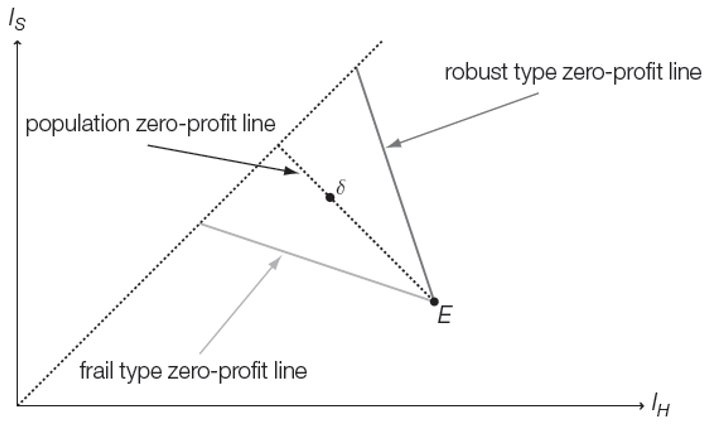
\includegraphics[width=0.8\textwidth]{./input/BHT_fig911.png}
    
\end{frame}
%---------------------------------------------------------------------
\begin{frame}{Different indifference curves}

    \begin{columns}[T]
        \begin{column}{0.5\textwidth}
            Utility curve for frail consumers are \textbf{steeper} than for robust consumers. \textit{Why?}\\
            \only<2>{$\implies$ Different \textbf{expected utilities} for the same contract}
        \end{column}
        \begin{column}{0.5\textwidth}
            \centering
            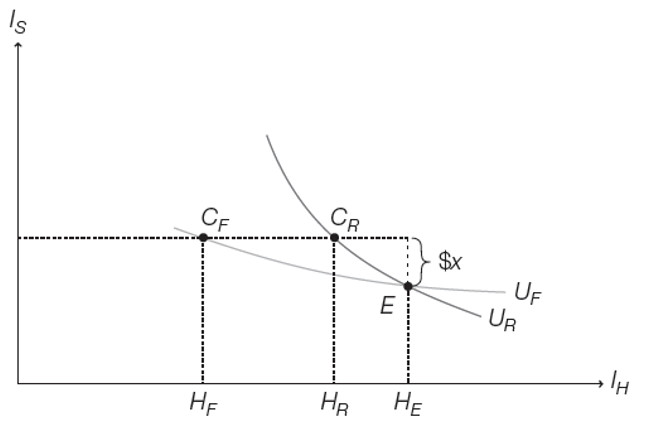
\includegraphics[width=\textwidth]{./input/BHT_fig912.png}
        \end{column}
    \end{columns}
    %Intuition: sick is less likely for robust, so willing to give less when healthy for increasing the unlikely sick state
    % EU = p U(I_S) + (1-p) U(I_H)
    % dEU = 0 \implies dI_S/dI_H = -[(1-p)·U'(I_H)] / [p·U'(I_S)]
    % Higher p $\implies$ lower dI_S/dI_H $\implies$ lower slope
    % That's the single crossing which is necessary in Spence and Mirlees (1978) for the existence of separating equilibrium

\end{frame}
%---------------------------------------------------------------------
\begin{frame}{Perfect information}

    \begin{columns}[T]
        \begin{column}{0.5\textwidth}
            Insurers \textbf{know} which type each consumer is:
            \begin{itemize}
                \item Frail consumers: offer $\Omega_1$
                \item Robust consumers: offer $\Omega_2$
            \end{itemize}
        \end{column}
        \begin{column}{0.5\textwidth}
            \centering
            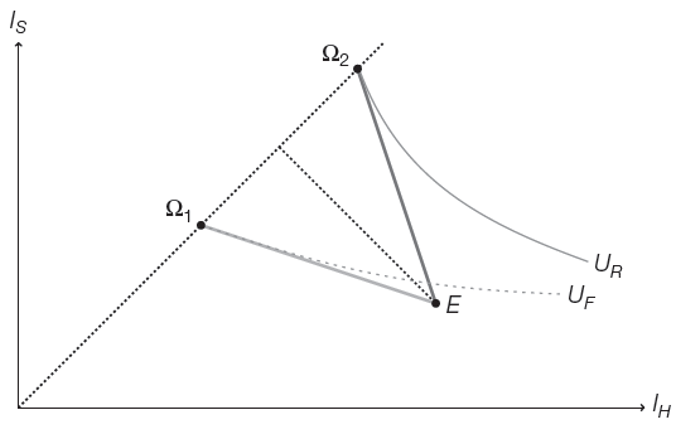
\includegraphics[width=\textwidth]{./input/BHT_fig914.png}
        \end{column}
    \end{columns}

\end{frame}
%---------------------------------------------------------------------
\begin{frame}{Now, introduce imperfect information}

    Now, assume the insurer cannot tell which consumer is frail and which consumer is robust
    $\implies$ \newbold{asymmetry of information} between consumers and insurers

\end{frame}
%---------------------------------------------------------------------
\begin{frame}{Pooling equilibrium}

    \newbold{Pooling equilibrium}: a contract that attracts both types of consumers \newbold{and} satisfies the equilibrium conditions\\
    \vspace{10mm}
    
    Does a pooling equilbrium exist in this model? \only<2>{\textbf{No.}}
\end{frame}
%---------------------------------------------------------------------
\begin{frame}{No pooling equilibrium}
    \begin{columns}[T]
        \begin{column}{0.4\textwidth}
            Is $\alpha$ a pooling equilibrium?
            \begin{enumerate}
                \item Higher utility for both types
                \item Population zero-profit for insurer
                \item \textbf{Could the insurer do better though?}
            \end{enumerate}
        \end{column}
        \begin{column}{0.6\textwidth}
            \centering
            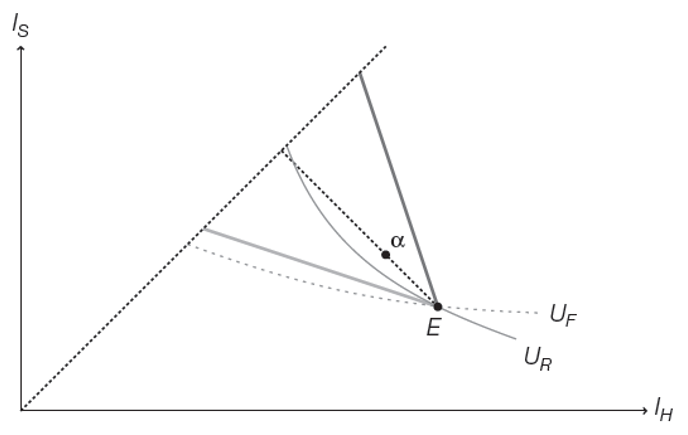
\includegraphics[width=\textwidth]{./input/BHT_fig915.png}
        \end{column}
    \end{columns}
\end{frame}
%---------------------------------------------------------------------
\begin{frame}{No pooling equilibrium}

    \begin{columns}[T]
        \begin{column}{0.4\textwidth}
            Exploit the triangle between the indifference curves. For example $\delta$:
            \begin{enumerate}
                \item Higher utility for robust, not for frail: frail don't buy
                \item Insurer offering $\delta$ makes positive profits from selling to robust only
            \end{enumerate}
            $\implies$ $\alpha$ only has frail, so insurers make negative profits\\
            $\implies$ $\alpha$ \newbold{is not} an equilibrium
        \end{column}
        \begin{column}{0.6\textwidth}
            \centering
            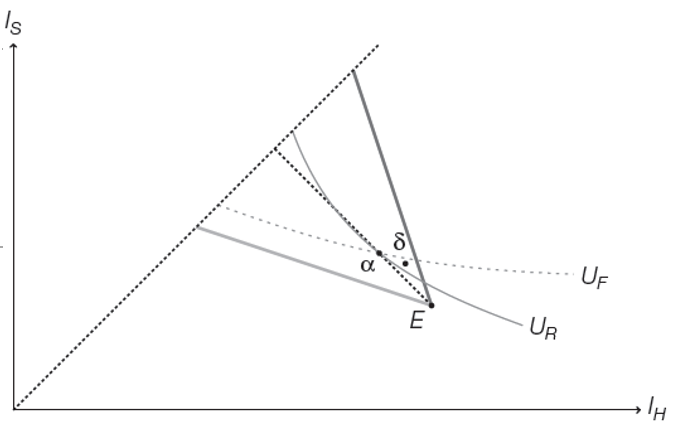
\includegraphics[width=\textwidth]{./input/BHT_fig916.png}
        \end{column}
    \end{columns}
    
\end{frame}
%---------------------------------------------------------------------
\begin{frame}{Separating equilibrium}

    \newbold{Separating equilibrium}: two contracts that each attract one type of consumers \textbf{and} both satisfy the equilibrium conditions\\
    \vspace{10mm}
    
    Does a separating equilibrium exist in this model? \only<2>{\textbf{Yes, but not always.}}
\end{frame}
%---------------------------------------------------------------------
\begin{frame}{A separating equilibrium}
    
    \begin{columns}[T]
        \begin{column}{0.5\textwidth}
            Is $(\Omega_1,\Omega_3)$ is a \newbold{separating equilibrium}?
            \only<2>{ \textbf{Yes!}
            \begin{enumerate}
                \item Zone $R_1$: only frail would prefer to $\Omega_3$ and insurer would make negative profits
                \item Zone $R_2$: both types would prefer but insurer would make negative profits
                \item Zone $R_3$: only robust would prefer to $\Omega_3$ but insurer would make negative profits
            \end{enumerate}
            }
        \only<1>{\vspace{48mm}}
        \end{column}
        \begin{column}{0.5\textwidth}
            \centering
            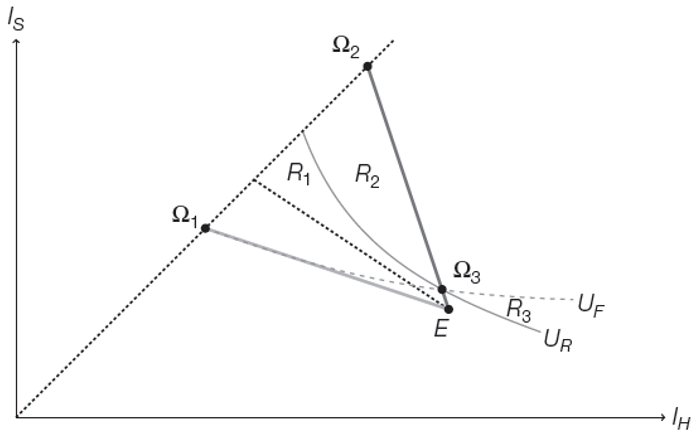
\includegraphics[width=\textwidth]{./input/BHT_fig917.png}
        \end{column}
    \end{columns}

\end{frame}
%---------------------------------------------------------------------
\begin{frame}{Who is hurt by asymmetric information?}

    Compare equilibria between perfect and imperfect information cases:
    \begin{itemize}
        \item Perfect information: frail choose $\Omega_1$ and robust choose $\Omega_2$
        \item Imperfect information: (if equilibrium exists) frail choose $\Omega_1$ and robust choose $\Omega_3$
    \end{itemize}
    \vspace{5mm}
    \pause

    $\implies$ \textbf{Frail consumers are indifferent}!!\\
    \pause
    $\implies$ Robust consumers are \textbf{worse off} with asymmetric information\\
    They are offered less than full insurance because of the presence of frail consumers in the population:
    ``externality'' of frail consumers on robust consumers
\end{frame}
%---------------------------------------------------------------------
\begin{frame}{When a separating equilibrium breaks down}

        \centering
        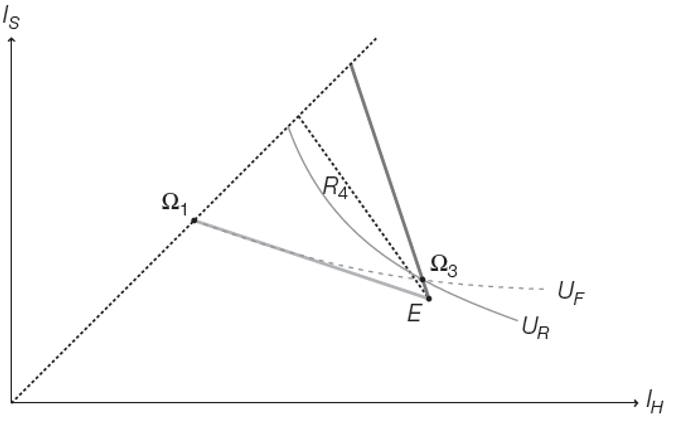
\includegraphics[width=0.7\textwidth]{./input/BHT_fig918.png}  

\end{frame}
%---------------------------------------------------------------------
\begin{frame}{When a separating equilibrium breaks down}

    \begin{columns}[T]
        \begin{column}{0.5\textwidth}
            What changed in this case: the population zero-profit line \textbf{is closer} to the robust zero-profit line\\
            $\implies$ there are more robust consumers in the population compared to frail consumers\\
            $\implies$ In the Rothschild-Stiglitz model, a separating equilibrium exists only if the \textbf{fraction of robust consumers is not ``too high''}
        \end{column}
        \begin{column}{0.5\textwidth}
            \centering
            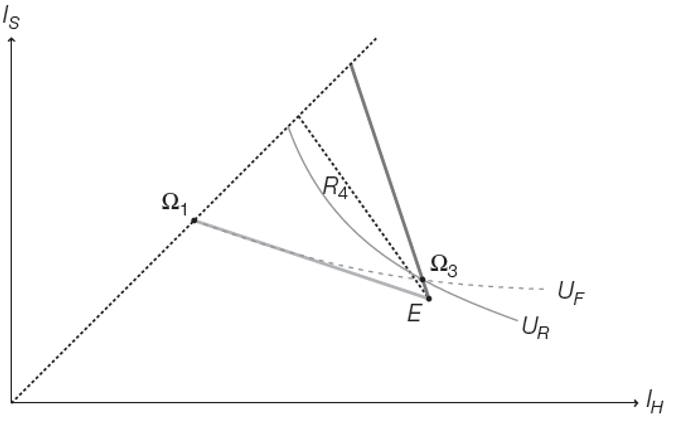
\includegraphics[width=\textwidth]{./input/BHT_fig918.png}
        \end{column}
    \end{columns}    

\end{frame}
%---------------------------------------------------------------------
\begin{frame}{Conclusion}

    The \newbold{Rothschild-Stiglitz model (1976)}
    \begin{itemize}
        \item Level of insurance and price can vary across contracts
        \item No pooling equilibrium, but separating equilibrium \textit{can} exist (but not always)
        \item Robust (healthy) consumers are worse off with asymmetric information, while frail (sick) consumers are indifferent
    \end{itemize} 
    
\end{frame}
%---------------------------------------------------------------------
\begin{frame}{Link to policy}

    Why is this model important/useful?
    \begin{itemize}
        \item Explains why insurers may offer different contract features\\
        $\implies$ \newbold{``cream skimming''}: use contract feature to attract or deter certain types of enrollees (screening device)
        \item It is more of a ``missing market'' distortion: do not cover some services to avoid attracting sick patients while patients would be willing to pay for it\\
        $\rightarrow$ narrow networks, restrictive drug formularies
        % We cut some coverage to avoid sick patients selecting into the plan, but this cuts coverage when people might want it and be willing to pay more for it.
        % Geruso Layton JEP 2017: exclude cancer coverage, both plans have cancer patients but cancer patients are poorly covered while they might be willing to pay more for coverage
        \item Policy tools: risk-adjustment and reinsurance, minimum health benefits
    \end{itemize}
\end{frame}
%---------------------------------------------------------------------
% \begin{frame}{}
%     \begin{center}
%     \Large \textcolor{maroon}{Optional Problem Set 1}
%     \end{center}
% \end{frame}
% %---------------------------------------------------------------------
% \begin{frame}{Instructions for optional problem set 1}

%     This is an \newbold{optional} problem set
%     \begin{itemize}
%         \item Due Thursday 03/19 by 9:30am
%         \item Bonus on your final grade: (0-not submitted, 1-submitted, 2-submitted and thoroughly done)
%         \item It is an empirical problem set making you use data and data analysis tools (e.g., Stata, R, or Python)\\
%     \end{itemize}
%     \vspace{5mm}

%     Two main angles:
%     \begin{enumerate}
%         \item Make you reproduce some figures in an empirical research paper
%         \item Check your understanding of some parts of the paper
%     \end{enumerate}
% \end{frame}
% %---------------------------------------------------------------------
% \begin{frame}{A quick look at the paper}

%     The paper:


%     Data

%     Empirical strategy


% \end{frame}
%---------------------------------------------------------------------
\begin{frame}{}
    \begin{center}
    \Large \textcolor{maroon}{Wrapping up}
    \end{center}
\end{frame}
%---------------------------------------------------------------------
\begin{frame}{To next class}
\begin{itemize}
    \item \newbold{TO DO}
    \begin{enumerate}
        \item \textbf{Enjoy spring break!}
        %\item \newbold{Optional problem set 1}: due \newbold{next Thursday 03/19 by 9:30am}
        \item Review this class and past material $\implies$ \textit{questions on it?}
    \end{enumerate}
    \vspace{5mm}

    \item After the break
    \begin{itemize}
        \item Continue on health insurance
        \item After midterm 2: move to the \textit{supply} of healthcare services 
    \end{itemize}
\end{itemize}
\end{frame}
%---------------------------------------------------------------------